%# -*- coding: utf-8-unix -*-
%%==================================================
\chapter{Spring}
\label{chap1}
\begin{itemize}[noitemsep,topsep=0pt,parsep=0pt,partopsep=0pt]
	\item ...
\end{itemize}

\section{知识点和方法论}

\subsection{知识点}
\subsubsection{jar 和 war 包之间的区别}
jar 包集成了Tomcat

war 没有集成Tomcat
\subsubsection{SpringBoot 和 SpringMVC 有什么区别}
SpringBoot 简化了项目的开发配置流程, 一定程度上消除了xml配置, 是一套快速配置开发的脚手架.

springMvc主要解决WEB开发的问题,是基于Servlet 的一个MVC框架,通过XML配置,统一开发前端视图和后端逻辑;

\subsubsection{Spring 框架能带来哪些好处}

\begin{enumerate}
	\item Dependency Injection(DI) 依赖注入 是的构造器和JavaBean properties文件中的依赖关系一目了然.
	\item IoC容器更加趋向于轻量级.
\end{enumerate}
\subsubsection{如何实现AOP, 项目那些地方用到了AOP}
利用JDK动态代理或Cglib动态代理, 利用动态代理技术, 可以针对某个类生成代理对象, 当调用代理对象的某个方法时, 可以任意控制该方法的执行, 比如可以先打印执行时间, 再执行该方法, 并且该方法执行完成后, 再次打印执行时间. \par
权限管理是使用AOP技术实现的. 凡是需要对某些方法做统一处理的都可以用AOP来实现, 利用AOP可以做到业务的无侵入 \par
\subsubsection{Spring的事物机制}
1. Spring事物机制底层是基于数据库事物和AOP机制的 \par
2. 首先对于使用了@Transactional注解的bean, spring会创建一个代理对象作为Bean \par
3. 当调用代理对象的方法时, 弧线判断方法上是否加了@Transactional注解 \par
4. 如果加了, 那么则利用事物管理器创建一个数据库连接 \par
5. 并且修改数据库连接的autocommit属性为false, 禁止此连接的自动提交, 这是实现Spring事物非常重要的一步. \par
6. 然后执行当前方法, 方法中会执行sql \par
7. 执行完当前方法后, 如果没有出现异常就直接提交事物 \par
8. 如果出现了异常, 并且这个异常是需要回滚的就会回滚事物, 否则仍然提交事物 \par
9. Spring事物的隔离级别对应的就是数据库的隔离级别 \par
10. Spring事物的传播机制是Spring事物自己实现的, 也是Spring事物中最复杂的. \par
11. Spring事物的传播机制是基于数据库连接来做的, 一个数据库连接一个事物, 如果传播机制配置为需要新开一个事物, 那么实际上就是先建立一个数据库连接, 在此新数据库连接上执行sql.
\subsubsection{Spring什么时候@Transactional失效}
如果某个纺纱是private的, 那么@Transactional也会失效, 因为底层cglib是基于父子类来实现的, 子类是不能重载父类的private方法的, 所以无法很好的利用代理, 也会导致@Transactional失效 \par
\subsubsection{介绍一下Spring, 读过源码介绍一下大致流程}
1. Spring是一个快速开发框架, Spring帮助程序员来管理对象 \par
2. Spring的源码实现的是非常优秀的, 设计模式的应用, 并发安全的实现, 面向接口的设计等 \par
3. 在创建Spring容器, 也就是启动Spring时: \par
a. 首先会进行扫描, 骚婊得到所有的BeanDefinition对象, 并存在一个Map中 \par
b. 然后筛选出非懒加载的单例BeanDefinition进行创建Bean, 对于多例Bean不需要再启动过程中去进行创建, 对于多例Bean会在每次获取Bean时利用beanDefinition去创建 \par
c. 利用beanDefinition创建Bean就是Bean的创建生命周期, 这期间包括了合并BeanDefinition, 推断构造方法, 实例化, 属性填充, 初始化前, 初始化, 初始化后等步骤, 其中AOP就是发生在初始化后这一步骤中\par
4. 单例Bean创建完了之后, Spring会发布一个容器启动事件. \par
5. Spring启动结束 \par

\subsubsection{Autowired}
使用byType和byName去寻找需要进行注入的对象
\subsubsection{什么是控制反转(IOC)}
\begin{enumerate}
	\item
	      控制反转简单来说, 以前程序开发的时候, 是由程序员通过new来生成对象. 在使用控制反转的情况下, 对象的实例化由Spring框架中的IoC容器来控制对象的创建;
	\item 由容器来管理这些对象的生命周期.
	\item Spring中的org.springframework.beans包和org.springframework.conext包构成了Spring框架Ioc的基础. 主要使用文件 applicationContext.xml 来进行配置.
\end{enumerate}

\subsubsection{什么是依赖注入?}
\begin{enumerate}
	\item Spring 通过反射来实现依赖注入
	\item 当我们需要某个功能比如Connection, 至于Connection怎么构造, 何时构造我们不需要知道. 在系统运行时, Spring会在适当的时候制造一个Connection, 我们需要一个Connection, 这个Connection是由Sping注入到A中.
\end{enumerate}
\subsubsection{Spring 对对象进行创建流程}
class对象反射 ---> 实例化 ---> 生成对象 ---> 属性填充(依赖注入)  ---> 初始化(afterPropertiesSet) ---> AOP ---> 代理对象(cglib) ---> bean
\subsubsection{什么是AOP}
允许横切业务, 由切面构成, 切面又切入点和通知构成,@Aspect注解的类就是切面. \par
(1) 目标对象(Target) \par
要被增强的对象. \par
(2) 连接点, 哪个目标方法, 相对点, 目标方法的前还是后.
\subsubsection{bean的生命周期}
什么是bean? \par
从上面可知,我们可以给Bean下一个定义:Bean就是由IOC实例化、组装、管理的一个对象。
\begin{figure}
	\centering
	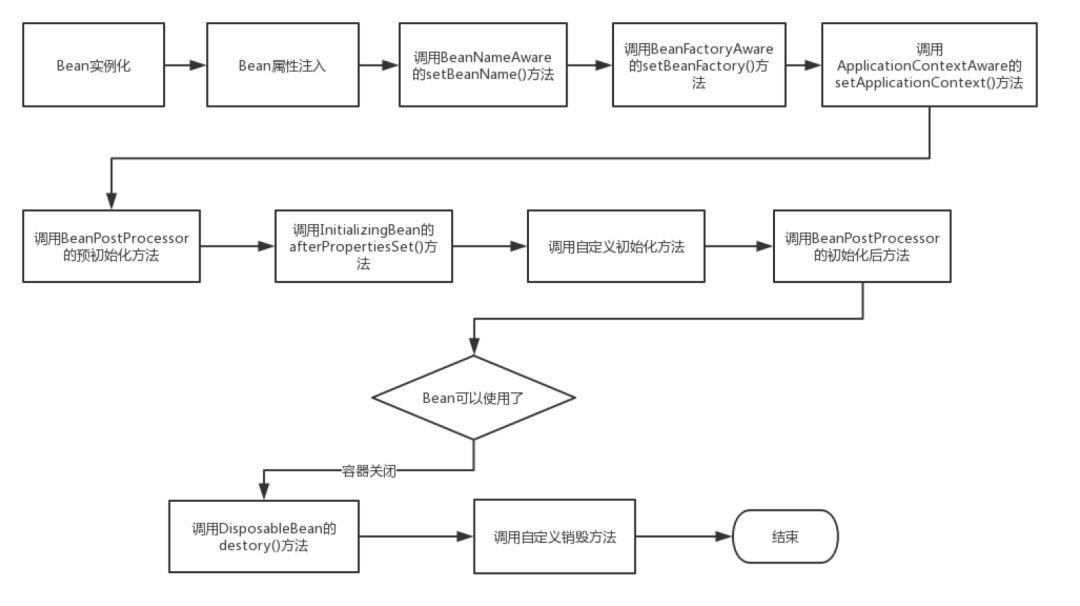
\includegraphics[width=0.7\linewidth]{figures/bean_live.jpg}
	\caption{beanlive}
	\label{fig:bean_live}

\end{figure}
如上图所示,Bean 的生命周期还是比较复杂的,下面来对上图每一个步骤做文字描述: \par
(1) Spring启动,查找并加载需要被Spring管理的bean,进行Bean的实例化 \par
(2) Bean实例化后对将Bean的引入和值注入到Bean的属性中 \par
(3) 如果Bean实现了BeanNameAware接口的话,Spring将Bean的Id传递给setBeanName()方法 \par
(4) 如果Bean实现了BeanFactoryAware接口的话,Spring将调用setBeanFactory()方法,将BeanFactory容器实例传入 \par
(5) 如果Bean实现了ApplicationContextAware接口的话,Spring将调用Bean的setApplicationContext()方法,将bean所在应用上下文引用传入进来。 \par
(6) 如果Bean实现了BeanPostProcessor接口,Spring就将调用他们的postProcessBeforeInitialization()方法。\par
(7) 如果Bean实现了InitializingBean接口,Spring将调用他们的afterPropertiesSet()方法。类似的,如果bean使用init-method声明了初始化方法,该方法也会被调用 \par

(8) 如果Bean 实现了BeanPostProcessor接口,Spring就将调用他们的postProcessAfterInitialization()方法。\par
(9) 此时,Bean已经准备就绪,可以被应用程序使用了。他们将一直驻留在应用上下文中,直到应用上下文被销毁。\par
(10) 如果bean实现了DisposableBean接口,Spring将调用它的destory()接口方法,同样,如果bean使用了destory-method 声明销毁方法,该方法也会被调用。\par
\subsubsection{简单阐述SpringMVC的流程}
SpringMVC是一个基于Java的实现了MVC设计模式的请求驱动类型的轻量级Web框架, 通过把Model, View, Controller分离, 将web层进行职责解耦, 把复杂的web应用分成逻辑清晰的几部分, 简化开发.
\par
(1) 用户发送请求到前端控制器DispatcherServlet;
\par
(2) DispatcherServlet 收到请求后, 调用HandlerMapping处理器映射器, 请求获取Handle
\par
(3) 处理器映射器更具请求url找到具体的处理器, 生成处理器对象以及处理器拦截器(如果有则生成)一并返回给DispatcherServlet;
\par
(4) DispatcherServlet 调用HandlerAdapter处理器适配器;
\par
(5) HandlerAdapter 经过适配调用具体处理器(Handler, 也叫后端控制器);
\par
(6) Handler 执行完成返回ModelAndView;
\par
(7) HandlerAdapter将Handler执行结果ModelAndView返回给DispatcherServlet;
\par
(8) DispatcherServlet将ModelAndView传给ViewResolver视图解析器进行解析;
\par
(9) ViewResolver解析后返回具体View
\par
(10) DispatcherServlet对View进行渲染视图(即将模型数据填充到视图中)
\par
(11) DispatcherServlet响应用户.
\par
简单来说, 我们需要开发的就是 == 开发处理器(Handler,即我们的Controller, 对于视图jsp我们前后端分离之后也不用写了.
\begin{figure}
	\centering
	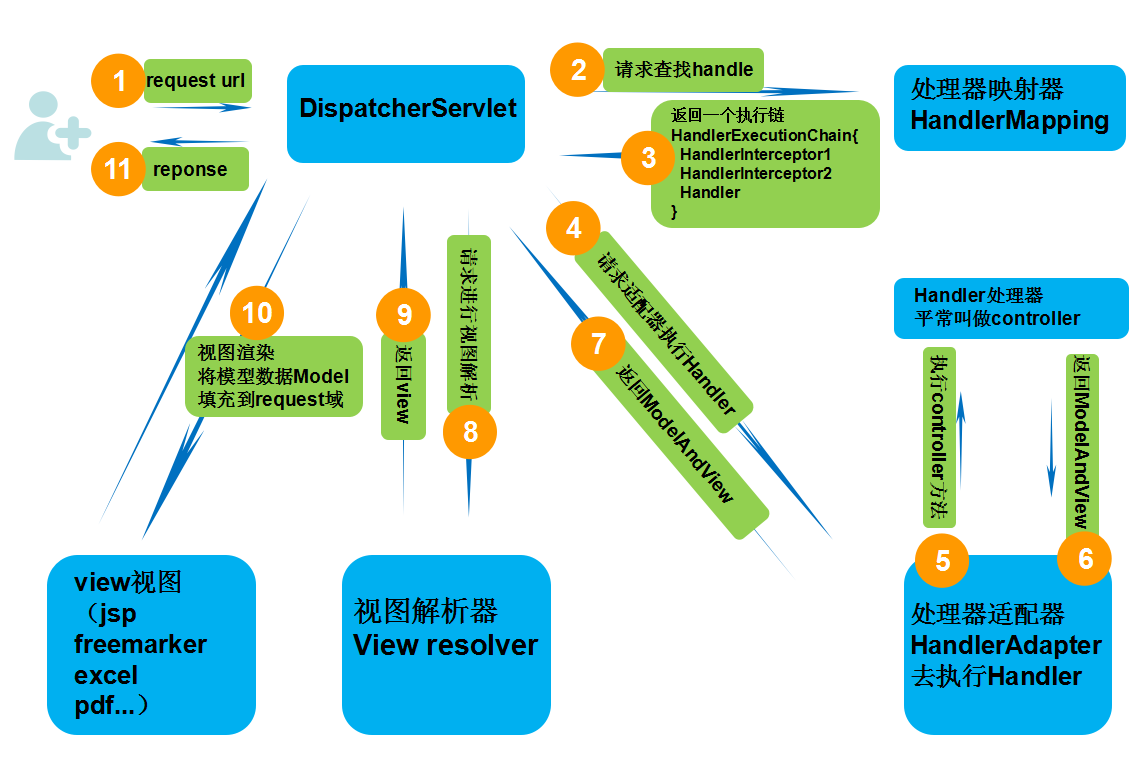
\includegraphics[width=0.7\linewidth]{figures/SpringModelAndView.png}
	\caption{SpringModelAndView}
	\label{fig:SpringModelAndView}
\end{figure}
\subsubsection{第三个三级标题}